\documentclass{article}
\usepackage{graphicx} % Required for inserting images
\usepackage{enumerate}
\usepackage{amssymb}
\usepackage[a4paper, total={6in, 8in}]{geometry}
\usepackage{hyperref}
\usepackage{amsmath}
\usepackage{amsthm}
\usepackage{cancel}
\usepackage{enumitem}

\usepackage{lastpage}
\usepackage{fancyhdr}
\usepackage{geometry}
\geometry{margin=1in}
\usepackage{underscore}
\usepackage{subcaption}
\usepackage{fancyvrb}
\usepackage{listings}
\lstset{basicstyle=\small\ttfamily, columns=flexible, breaklines=true}
\usepackage{tabularx}
\usepackage{float}
\usepackage{makecell}

\usepackage{mdframed}
\usepackage{lipsum}

\usepackage{hyperref}
\usepackage{multicol}
\usepackage{fancyhdr}
\pagestyle{fancy}
\fancyhf{} % Clear default headers and footers

% Add a simple header
\fancyhead[L]{\textbf{CSE-103 Notes}} % Left-aligned header text
\fancyhead[R]{\textbf{Spring 2025}}   % Right-aligned header text

% Add page numbers in the footer
\fancyfoot[C]{\thepage\ of \pageref{LastPage}} % Center-aligned footer with total pages

% Disable red box around page numbers (using hyperref)
\hypersetup{
    colorlinks=false, % Enable colored links
    linkcolor=blue,  % Set the color of internal links (like page numbers)
    urlcolor=blue,   % Set the color of URLs
    pdfborder={0 0 0} % Remove the border around links
}

% Set the listings font to a darker monospaced font (closer to Sipser's font)


\usepackage{tikz,tcolorbox}
\usepackage{xcolor}
\usepackage{newtxtext,newtxmath}

\usepackage{times,latexsym,mathptmx,comment,latexsym,epsf,amssymb,graphicx,url,enumerate}
\usetikzlibrary{arrows,positioning,automata}
\usetikzlibrary{arrows.meta}


\title{CSE-103: Computational Models\\ Lecture Notes}
\author{Mann Malviya}
\date{Spring 2025}

\begin{document}
\maketitle
\tableofcontents
\newpage

\section*{Introduction}
\addcontentsline{toc}{section}{Introduction} 


\subsection*{Textbooks}
\addcontentsline{toc}{subsection}{Textbooks} 

\begin{enumerate}
    \item Introduction to the Theory of Computation by Michael Sipser
    \begin{figure}[H]
        \centering
        
\includegraphics[scale=2]{103_TB.png}
        \caption*{\centering{Introduction to the Theory of Computation \\by Michael Sipser}}
    \end{figure}
\end{enumerate}

\begin{center}
	\rule{450pt}{1pt} 
\end{center}

\subsection*{What is this Doc?}
\addcontentsline{toc}{subsection}{What is this Doc?}
This document shall contain my notes for the class CSE-103: Computational Models offered at UCSC, taught by Assistant Prof. Daniel Fremont. This document will contain notes from the lectures(possibly verbatim?) and may contain some additional information, either from the text or other sources that I find useful.


\begin{center}
	\rule{450pt}{3pt} 
\end{center}
\newpage



\section*{Lecture 1}
\addcontentsline{toc}{section}{Lecture 1}

\subsection*{Overview of the Course}
\addcontentsline{toc}{subsection}{Overview of the Course}
\begin{itemize}
    \item This course is called \textbf{Computational Models} what does that actually mean?
    \begin{itemize}[label=\textbullet]
        \item SW    
    \end{itemize}
\end{itemize}



\subsection*{Learning Objectives}
\addcontentsline{toc}{subsection}{Learning Objectives}
After taking this course, you will be able to:
\begin{enumerate}
    \item Interpret and design finite automata (DFAs and NFAs) and regular expressions.
    \item Interpret and design context-free grammars (CFGs) and pushdown automata.
    \item Prove basic properties of regular and context-free languages.
    \item Interpret and design Turing machines(TMs).
    \item Prove basic languages are decidable or Turing-recognizable.
    \item Construct reductions between problems and apply such reductions to establish undecidability of problems
    \item Construct polynomial-time algorithms/verifiers and polynomial-time reductions and use them to show languages are in P, NP, or are NP-complete.
\end{enumerate}


\subsection*{Outline of the Course}
\addcontentsline{toc}{subsection}{Outline of the Course}

\begin{center}
	\rule{450pt}{1pt} 
\end{center}
\newpage

\section*{Lecture 2:}
\addcontentsline{toc}{section}{Lecture 2}

We are building up to a simple model of computation: The Finite Automaton.

\subsection*{What is Computation?}
\addcontentsline{toc}{subsection}{What is Computation?}
\begin{itemize}
    \item A computation is some kind of procedure that takes some input and produces some output.
    \begin{figure}[H]
        \centering{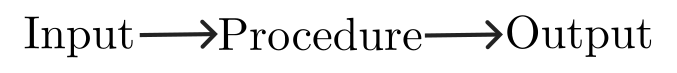
\includegraphics[scale=1.5]{computation.png}}
        \caption*{A Computation}
    \end{figure}
    \item We will talk about how we can model each of the 3 parts, the \textbf{input}, the \textbf{procedure}, and the \textbf{output}.
\end{itemize}

\subsection*{Input}
\addcontentsline{toc}{subsection}{Input}

\begin{figure}[H]
    \centering{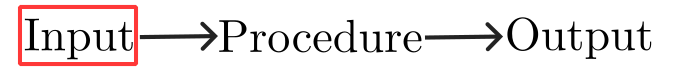
\includegraphics[scale=1.5]{Input.png}}
    \caption*{}
\end{figure}

\begin{itemize}
    \item The input will always be a finite sequence of symbols, e.g. "001101" or "abca".
    
    \begin{tcolorbox} [title= Definition:, colback=black!10!white]
        The set of allowed symbols is called the \textbf{alphabet} (by analogy to natural language) and is denoted by $\Sigma$.
    \end{tcolorbox}
    \begin{itemize}
        \item[$	$] Example: The binary alphabet $\{0,1\}$
    \end{itemize}
    \item The only thing we will assume about the \textbf{alphabet} $\Sigma$ is that it's finite.
    \begin{tcolorbox} [title= Definition:, colback=black!10!white]
        A \textbf{string} or \textbf{word} over $\Sigma$ is a finite sequence of symbols from $\Sigma$.
    \end{tcolorbox}
    \begin{itemize}
        \item[$ $] Example: 00, 101, 000 are words over the binary alphabet.
    \end{itemize}
    \item These words/strings are going to be the inputs to the algorithms we will talk about in this class, one could imagine there are plenty of algorithms that operate on other kinds of input, like images, sounds, videos etc. but you can find ways of encoding them in binary. Then you can treat any arbitrary kind of input as being a finite sequence of 0's and 1's.
    \item If $w$ is a string, $|w|$ is the no. of symbols in $w$.
    \begin{itemize}
        \item[$ $] Example: $|110|=3$
    \end{itemize}
    \item The empty string is denoted by $\varepsilon$ and has a length zero i.e., $|\varepsilon|=0$.
    \item When given a string, $w$ if you want to refer to an individual symbol within the sting then you do so by $w_i$, for any $i$ between $1$ and $|w|$ (i.e., $1\le i \le |w|$), $w_i$ is the $i^{\text{th}}$ symbol of $w$. We are indexing starting from $1$, this is just a convention.
    \begin{itemize}
        \item [$ $] Example: $w=110$ then $w_1=1$, $w_2=1$, $w_3=0$.
    \end{itemize}
    \item Another very common operation we will need to use on strings is \textbf{concatenation} which is taking 2 strings and joining them together. We write concatenation as multiplication, so $w=xy$ means $w$ consists of the symbol of $x$ followed by the symbols of $y$.
    \begin{itemize}
        \item [$ $] Example: $x=001$ and $y=10$ then $xy=00110$ and $yx=10001$. Notice that concatenation is not commutative.
    \end{itemize}
    \begin{tcolorbox} [title= Definition:, colback=black!10!white]
        For any non-negative($\ge 0$) integer $k$, i.e., $k\in\mathbb{Z}^+$, $\Sigma^k$ is the set of all strings over $\Sigma$ of length $k$.
    \end{tcolorbox}
    \begin{itemize}
        \item[$ $] Example: $\{0,1\}^2=\text{all length 2 binary strings} = \{00,01,10,11\}$
    \end{itemize} 
    \item We write $\Sigma^{\le k}$ for the set of strings over $\Sigma$ of length $\le k$. 
    \begin{itemize}
        \item [$ $] Example: if $\Sigma=\{0,1\}$ then,
        \begin{align*}
            \Sigma^{\le 2} &= \Sigma^0 \cup \Sigma^1 \cup \Sigma^2 \\
                           &= \{\varepsilon\} \cup \{0,1\} \cup \{00,01,10,11\} \\
                           &= \{\varepsilon, 0, 1, 00, 01, 10, 11\}
        \end{align*}
        

    \end{itemize}
    \item[$ $] \underbar{Note}: For any alphabet $\Sigma$, $\Sigma^0$ is the set of words of length zero, of which there is exactly one: the empty string $\varepsilon$.
    $$\Sigma^0 = \{\varepsilon\}\neq\varnothing$$
    \item We write $\Sigma^*$(sigma-star) for the set of all strings of any length over $\Sigma$. Formally, $$\Sigma^*=\bigcup_{k\ge0}\Sigma^k$$
    This is an infinite set.
    \begin{itemize}
        \item [$ $] Example: $\{0,1\}^*=\{\varepsilon, 0, 1, 00, 01, 10, 11, 000,...\}$
    \end{itemize}
\end{itemize}

\

\noindent This is going to suffice for us to talk about the input to our algorithms, because we will just assume some kind of standardized encoding of all other kinds of inputs into binary strings. The details of how we do the encoding will not be important at least in this class.

We will assume a standardized binary encoding of non-string datatypes, so that we can treat all inputs as binary strings. This shouldn't be too hard to believe because on real computers, everything is stored as $0$ and $1$'s anyways.

\

{\large \textbf{Exercise:}}
\begin{enumerate}
    \item How many elements are in the set $\{a,b,c\}^3$?
    \item How many elements are in the set $\{a\}^3$?
\end{enumerate}



\subsection*{Output}
\addcontentsline{toc}{subsection}{Output}
\begin{figure}[H]
    \centering{
\includegraphics[scale=1.5]{output.png}}
    \caption*{}
\end{figure}

\begin{itemize}
    \item We will make a somewhat restrictive assumption, we are only going to look at algorithms who's answer is YES/NO or TRUE/FALSE\footnote{For the purposes of this class, it's sufficient for us to just deal with TRUE/FALSE questions, not too much interesting new stuff happens if you consider more complicated things, so we will not worry about that here.}. These are called \textbf{decision problems}. In these kinds of problems we are simply trying to say YES or NO, we are not going to deal with problems that need a string output. 
    \begin{tcolorbox} [title= Definition:, colback=black!10!white]
        Problems for which every possible inputs output is either YES or NO are called \textbf{decision problems}.
    \end{tcolorbox}
    \begin{itemize}
        \item[$ $] Example: "Does a binary string contain an even number of $1$'s" is a Decision problem
        \begin{align*}
            011 &\rightarrow \text{YES}\\ 
            0100 &\rightarrow \text{NO}\\
            \varepsilon &\rightarrow \text{YES}
        \end{align*}  
    \end{itemize}
    \begin{tcolorbox} [title= Definition:, colback=black!10!white]
        To fully specify a decision problem, it's enough to identify the strings with answers "YES", this set is called the \textbf{language}\footnotemark{} of the decision problem. A language $\mathcal{L}$ over an alphabet $\Sigma$ is a subset, $\mathcal{L}\subseteq\Sigma^*$.
    \end{tcolorbox}
    \item The decision problem for $\mathcal{L}$ is to decide whether a given string $w\in\Sigma^*$ is in $\mathcal{L}$, i.e. $w\in\mathcal{L}$?
    \begin{itemize}
        \item [$ $] Example: $\mathcal{L}_{\text{PRIME}}=\text{"binary string encoding prime numbers"}$
        \begin{align*}
            10 &\in\mathcal{L_\text{PRIME}}\\
            101 &\in\mathcal{L_\text{PRIME}}\\
            1001 &\notin\mathcal{L_\text{PRIME}}\\
        \end{align*}
    \end{itemize}
\end{itemize}

\footnotetext{because it's a set of words, an analogy from natural language}

\subsection*{Procedure}
\addcontentsline{toc}{subsection}{Procedure}
\begin{figure}[H]
    \centering{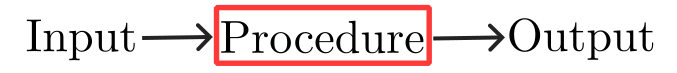
\includegraphics[scale=1.5]{procedure.png}}
    \caption*{}
\end{figure}

\begin{itemize}
    \item In a decision problem, you take in a finite string as input and you need to output either YES or NO, one question is how do you make the decision? Thats where the computational model is going to come in, you can think of the \textbf{procedure} as just a way of computing the mapping from inputs to outputs.
    \begin{tcolorbox} [title= Definition:, colback=black!10!white]
        The \textbf{procedure} is a mapping from the inputs to the outputs.
    \end{tcolorbox}
    \item You can model the procedure mathematically as just a function, because thats what a function does, it tells you for every possible input, what the output is.
    \item In general the function can be written as, $$f:\Sigma^*\rightarrow\{\underset{\text{no}}{0},\underset{\text{yes}}{1}\}$$
    The language $\mathcal{L}$ for $f$ would be the set of all inputs $x$ such that $f\left(x\right)=1$, $$ \mathcal{L}=\{x\in\Sigma^*|f(x)=1\}$$
    \underbar{Note}: A well defined function need not have an actual algorithm for computing $f\left(x\right)$ from $x$.
    \begin{itemize}
        \item [$ $] Example: 
        $$
            f\left(x\right) =
            \begin{cases}
                1 & \text{if x encodes a python program that terminates}\\
                0 & \text{otherwise}
            \end{cases}
        $$
        Later we will see that this function is \textbf{not} computed by any algorithm.
    \end{itemize}
\end{itemize}

Next lecture we will define \textbf{finite automata} as a restricted class of such functions.

\subsection*{Exercise Solutions}
\addcontentsline{toc}{subsection}{Exercise Solutions}
\begin{enumerate}
    \item 3 symbols to pick since we want to find $|\Sigma^3|$ which only contains words of length 3, we have 3 options fore each symbol($a$,$b$ or $c$) so by the multiplication principle from combinatorics, we have $3\cdot3\cdot3=3^3=27$ words of length 3.
    \item $|\{a\}^3|=1^3=1$
\end{enumerate}

\begin{center}
	\rule{450pt}{1pt} 
\end{center}
\newpage

\section*{Lecture 3:}
\addcontentsline{toc}{section}{Lecture 3}
Last Lecture we spoke about the process of going from an input to an output(the procedure) we going to talk about several such models, the first being \textbf{Finite Automata}.

\subsection*{Finite Automata}
\addcontentsline{toc}{subsection}{Finite Automata}

\begin{itemize}
    \item We will first cover the intuition for finite automata and then cover the formal definition.
    \item Intuition: Think of finite automata as "computers" with limited memory.
    \item Programming languages like C/C++ provide mechanisms to allocate new memory, but in finite automaton you cannot do that, you have a fixed amount of memory which is set once and for all and it's independent of the size of the input given.
    \item There's a convenient way to draw finite automata as directed graphs, representing each state as a node and the arrows/edges between them as transitions, with each edge labeled with the input symbol that causes the transition.
    \begin{itemize}
    \item Let $M$ be a machine that reads an input string one symbol at a time.
    \item The machine $M$ has a \textbf{finite} number of modes or states.
    \item The machine $M$ remembers things by being in different states.
    \item The machine \textbf{transitions} to the next state based on the input symbol and the current state.
    \item After reaching all symbols, $M$ \textbf{accepts}(answer YES) if we end up in an "accepting state" otherwise it \textbf{rejects}(answer NO).
    \end{itemize}
\end{itemize}

\subsection*{Examples of Finite Automata}
\addcontentsline{toc}{subsection}{Examples of Finite Automata}

\subsection*{Deterministic Finite Automata (DFA)}
\addcontentsline{toc}{subsection}{Deterministic Finite Automata (DFA)}

\tikzset{accepting/.style={accepting by double, double distance=3pt}}

The following is all the state machines drawn in this lecture:

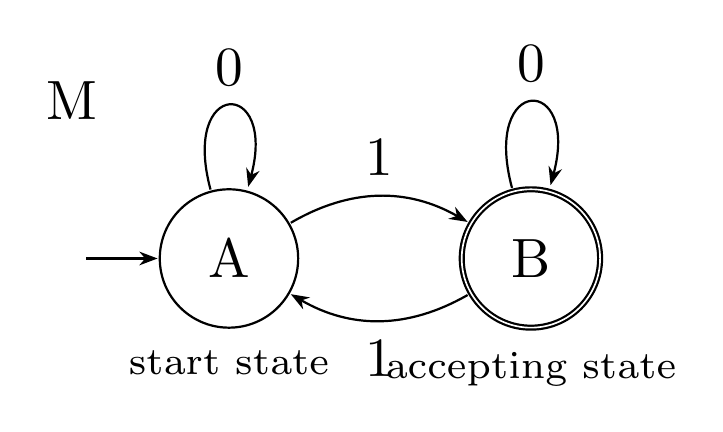
\begin{tikzpicture}[scale=2, transform shape, 
    >=Stealth, 
    every path/.style={->, >=Stealth, thick}, 
    tip/.style={scale=1.5}] 
    \node at (-1, 1) {M};
    \node[state, initial, initial text=] (s1) {A};
    \node[below=0cm of s1] {\scriptsize start state};
    \node[state, accepting, right= of s1] (s2) {B};
    \node[below=0cm of s2] {\scriptsize accepting state};
    \path[->]
        (s1) edge[bend left] node[above] {$1$} (s2)
        (s1) edge[loop above] node[above] {$0$} (s1)
        (s2) edge[bend left] node[below] {$1$} (s1)
        (s2) edge[loop above] node[above] {$0$} (s2)
        ;
\end{tikzpicture}

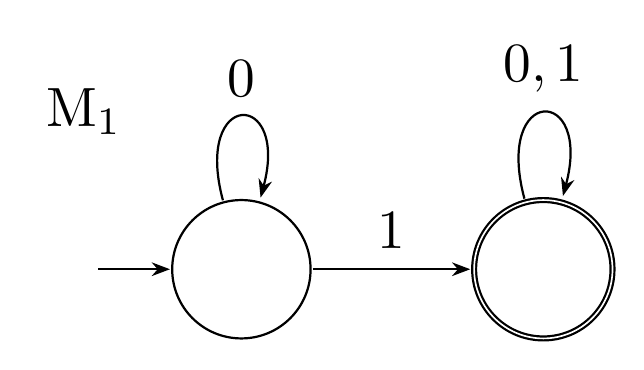
\begin{tikzpicture}[scale=2, transform shape, 
    >=Stealth, 
    every path/.style={->, >=Stealth, thick}, 
    tip/.style={scale=1.5}] 
    \node at (-1, 1) {$\text{M}_1$};
    \node[state, initial, initial text=] (s1) {};
    \node[state, accepting, right= of s1] (s2) {};
    \path[->]
        (s1) edge[right] node[above]{$1$} (s2)
        (s1) edge[loop above] node[above]{$0$} (s1)
        (s2) edge[loop above] node[above]{$0,1$} (s2)
        ;
\end{tikzpicture}

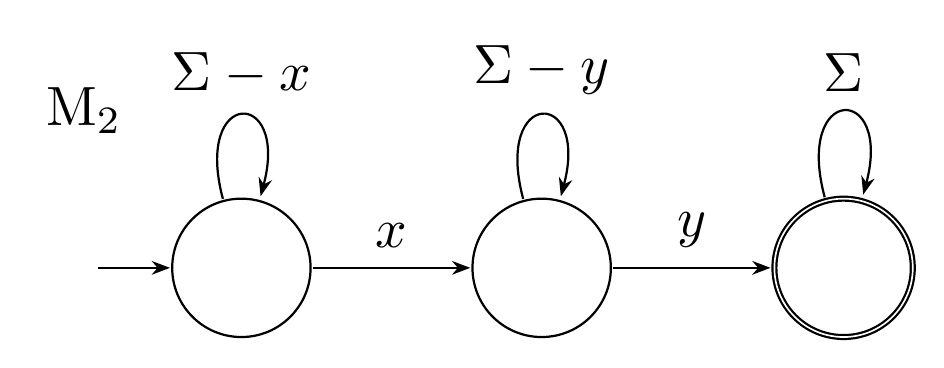
\begin{tikzpicture}[scale=2, transform shape, 
    >=Stealth, 
    every path/.style={->, >=Stealth, thick}, 
    tip/.style={scale=1.5}] 
    \node at (-1, 1) {$\text{M}_2$};
    \node[state, initial, initial text=] (s1) {};
    \node[state, right= of s1] (s2) {};
    \node[state, accepting, right= of s2] (s3) {};
    \path[->]
        (s1) edge[right] node[above]{$x$} (s2)
        (s2) edge[right] node[above]{$y$} (s3)
        (s1) edge[loop above] node[above]{$\Sigma-x$} (s1)
        (s2) edge[loop above] node[above]{$\Sigma-y$} (s2)
        (s3) edge[loop above] node[above]{$\Sigma$} (s3)
    ;
\end{tikzpicture}

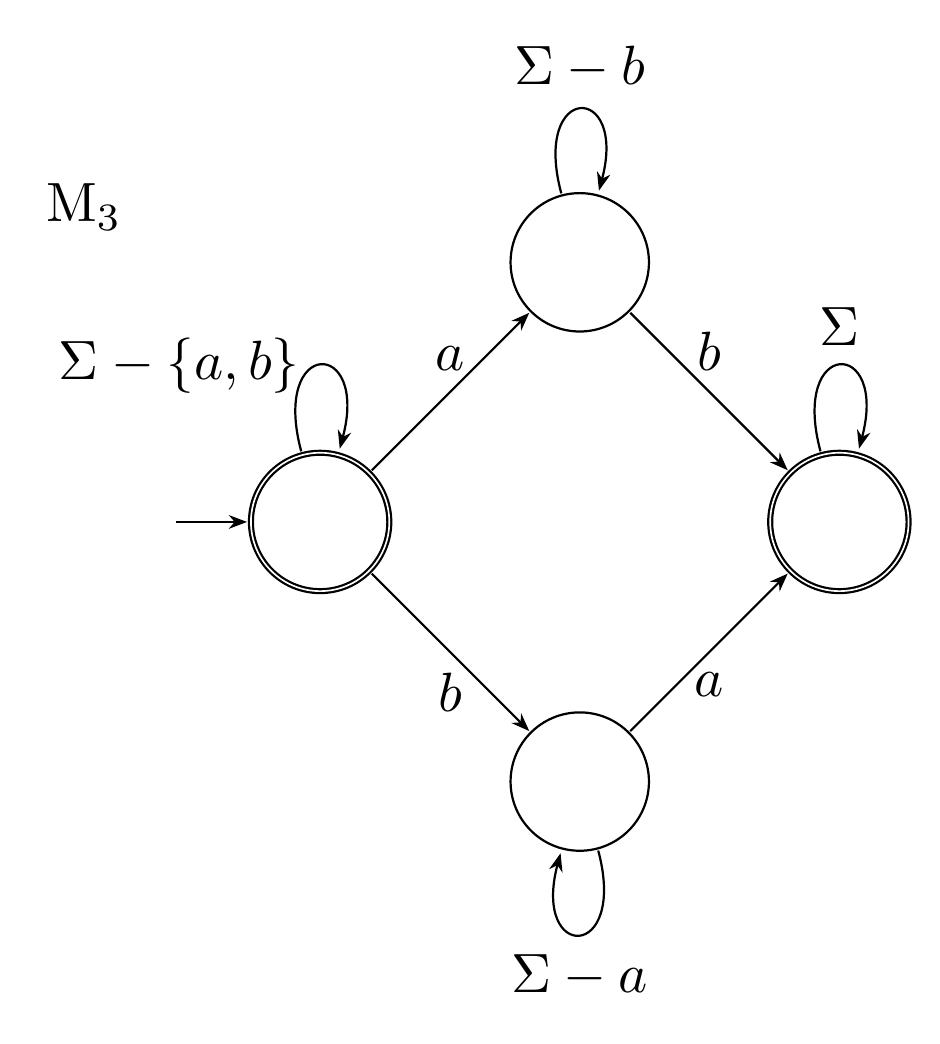
\begin{tikzpicture}[scale=2, transform shape, 
    >=Stealth, 
    every path/.style={->, >=Stealth, thick}, 
    tip/.style={scale=1.5}] 
    \node at (-1.5, 2) {$\text{M}_3$};
    \node[state, accepting, initial, initial text=] (s1) {};
    \node[state, above right= of s1] (s2) {};
    \node[state, below right= of s1] (s3) {};
    \node[state, accepting, below right= of s2] (s4) {};
    \path[->]
        (s1) edge[loop above] node[left]{$\Sigma-\{a,b\}$} (s1)
        (s1) edge[] node[above]{$a$} (s2)
        (s1) edge[] node[below]{$b$} (s3)
        (s2) edge[loop above] node[above]{$\Sigma-b$} (s2)
        (s2) edge[] node[above]{$b$} (s4)
        (s4) edge[loop above] node[above]{$\Sigma$} (s4)
        (s3) edge[loop below] node[below]{$\Sigma-a$} (s3)
        (s3) edge[] node[below]{$a$} (s4)
        ;
\end{tikzpicture}



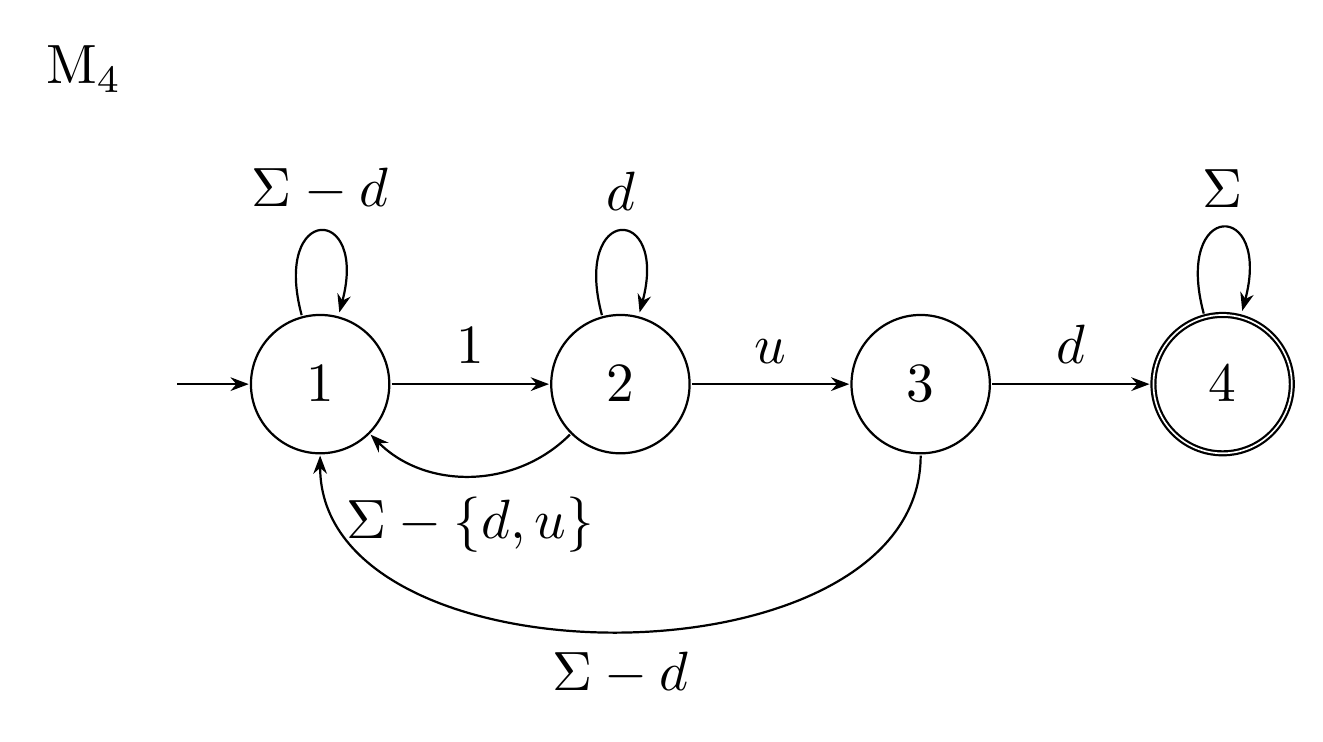
\begin{tikzpicture}[scale=2, transform shape, 
    >=Stealth, 
    every path/.style={->, >=Stealth, thick}, 
    tip/.style={scale=1.5}] 
    \node at (-1.5, 2) {$\text{M}_4$};
    \node[state, initial, initial text=] (s1) {1};
    \node[state, right= of s1] (s2) {2};
    \node[state, right=of s2] (s3) {3};
    \node[state, accepting, right=of s3] (s4) {4};
    \path[->]
        (s1) edge[loop above] node[above]{$\Sigma-d$} (s1)
        (s1) edge[] node[above]{\lstinline{1}} (s2)
        (s2) edge[loop above] node[above]{$d$} (s2)
        (s2) edge[] node[above]{$u$} (s3)
        (s2) edge[bend left=45] node[below]{$\Sigma-\{d,u\}$} (s1)
        (s3) edge[bend left=90] node[below]{$\Sigma-d$} (s1)
        (s3) edge[] node[above]{$d$} (s4)
        (s4) edge[loop above] node[above]{$\Sigma$} (s4)
        ;
\end{tikzpicture}

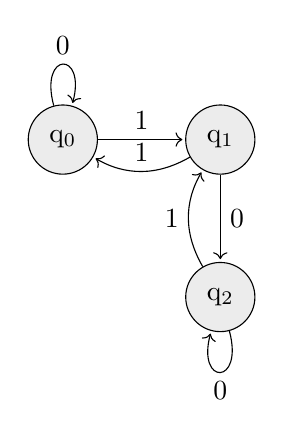
\begin{tikzpicture}[shorten >=1pt, node distance=2cm, on grid, auto]
    % Define states with a grey fill
    \node[state, fill=gray!15, text=black] (q_0)   {q$_0$}; 
    \node[state, fill=gray!15, text=black, right=of q_0] (q_1) {q$_1$};
    \node[state, fill=gray!15, text=black, below=of q_1] (q_2) {q$_2$};
    
    % Define the initial and accepting states
    \path[->]
    (q_0) edge [loop above] node {\lstinline{0}} ()
          edge node {1} (q_1)
    (q_1) edge node {0} (q_2)
          edge [bend left, above] node {\lstinline{1}} (q_0)
    (q_2) edge [bend left, below] node[left] {\lstinline{1}} (q_1)
          edge [loop below] node {\lstinline{0}} ();
\end{tikzpicture}





\begin{center}
	\rule{450pt}{1pt} 
\end{center}
\newpage

\section*{Lecture 4:}
\addcontentsline{toc}{section}{Lecture 4}

\subsection*{DFAs continued}
\addcontentsline{toc}{subsection}{DFAs continued}

\subsection*{A proof using PMI}
\addcontentsline{toc}{subsection}{A proof using PMI}

\subsection*{Extended transition function}
\addcontentsline{toc}{subsection}{Extended transition function}

\begin{center}
	\rule{450pt}{1pt} 
\end{center}
\newpage


\section*{Lecture 5:}
\addcontentsline{toc}{section}{Lecture 5}

\subsection*{Extended transition function continued}
\addcontentsline{toc}{subsection}{Extended transition function continued}


\subsection*{Some Definitions}
\addcontentsline{toc}{subsection}{Some Definitions}

\subsection*{Nondeterministic Finite Automata (NFA)}
\addcontentsline{toc}{subsection}{Nondeterministic Finite Automata (NFA)}

The following is all the state machines drawn in this lecture:

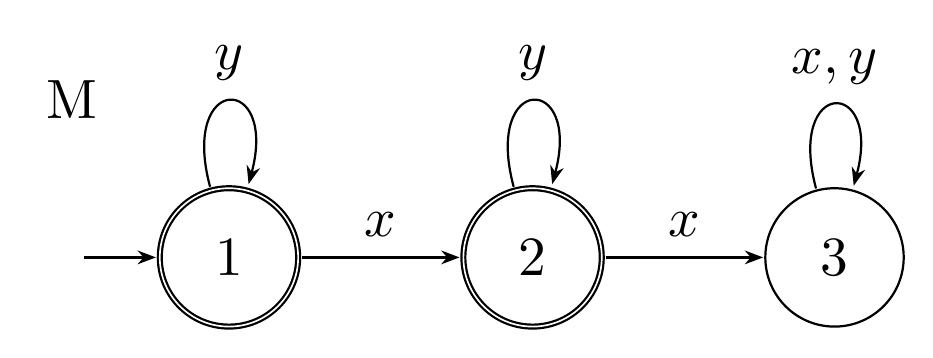
\begin{tikzpicture}[scale=2, transform shape, 
    >=Stealth, 
    every path/.style={->, >=Stealth, thick}, 
    tip/.style={scale=1.5}] 
    \node at (-1, 1) {M};
    \node[state, accepting, initial, initial text=] (s1) {$1$};
    \node[state,accepting, right= of s1] (s2) {$2$};
    \node[state, right= of s2] (s3) {$3$};
    \path[->]
        (s1) edge[loop above] node[above]{$y$} (s1)
        (s1) edge[] node[above]{$x$} (s2)
        (s2) edge[loop above] node[above]{$y$} (s2)
        (s2) edge[] node[above]{$x$} (s3)
        (s3) edge[loop above] node[above]{$x,y$} (s3)
        ;
\end{tikzpicture}

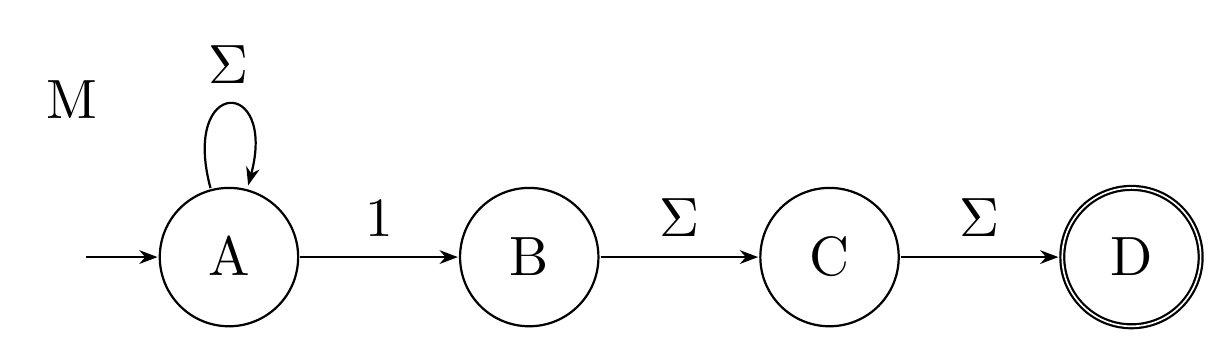
\begin{tikzpicture}[scale=2, transform shape, 
    >=Stealth, 
    every path/.style={->, >=Stealth, thick}, 
    tip/.style={scale=1.5}] 
    \node at (-1, 1) {M};
    \node[state, initial, initial text=] (s1) {A};
    \node[state, right= of s1] (s2) {B};
    \node[state, right= of s2] (s3) {C};
    \node[state, accepting, right= of s3] (s4) {D};
    \path[->]
        (s1) edge[loop above] node[above]{$\Sigma$} (s1)
        (s1) edge[] node[above]{$1$} (s2)
        (s2) edge[] node[above]{$\Sigma$} (s3)
        (s3) edge[] node[above]{$\Sigma$} (s4)
        ;
\end{tikzpicture}

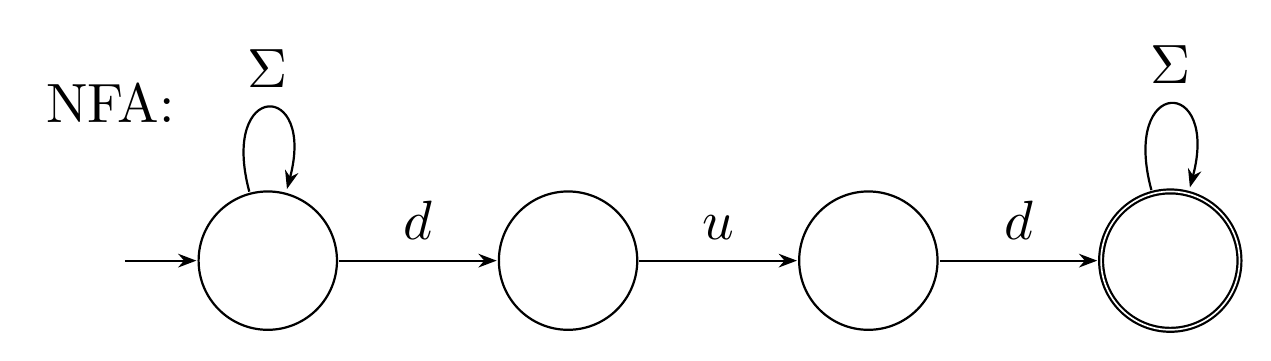
\begin{tikzpicture}[scale=2, transform shape, 
    >=Stealth, 
    every path/.style={->, >=Stealth, thick}, 
    tip/.style={scale=1.5}] 
    \node at (-1, 1) {NFA:};
    \node[state, initial, initial text=] (s1) {};
    \node[state, right= of s1] (s2) {};
    \node[state, right= of s2] (s3) {};
    \node[state, accepting, right= of s3] (s4) {};
    \path[->]
        (s1) edge[loop above] node[above]{$\Sigma$} (s1)
        (s1) edge[] node[above]{$d$} (s2)
        (s2) edge[] node[above]{$u$} (s3)
        (s3) edge[] node[above]{$d$} (s4)
        (s4) edge[loop above] node[above]{$\Sigma$} (s4)
        ;
\end{tikzpicture}

\begin{center}
	\rule{450pt}{1pt} 
\end{center}
\newpage

\section*{Lecture 6:}
\addcontentsline{toc}{section}{Lecture 6}

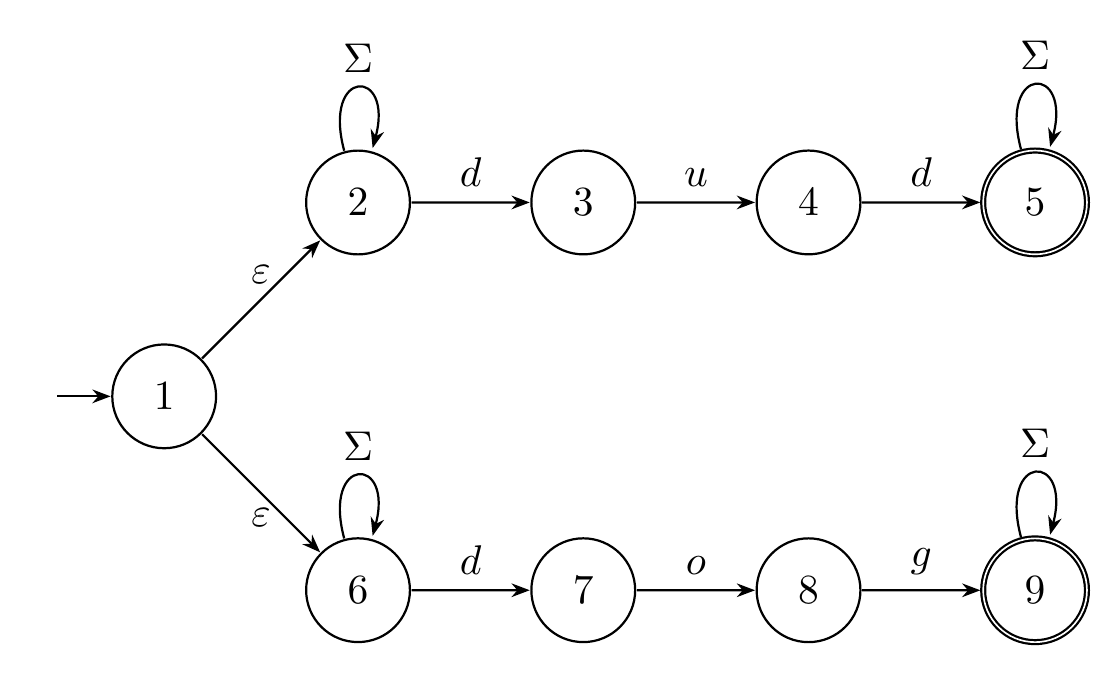
\begin{tikzpicture}[scale=1.5, transform shape, 
    >=Stealth, 
    every path/.style={->, >=Stealth, thick}, 
    tip/.style={scale=1.5}] 
    \node [state, initial, initial text=] (s1) {1};
    \node[state, above right= of s1] (s2) {2};
    \node[state, right= of s2] (s3) {3};
    \node[state,right= of s3] (s4) {4};
    \node[state, accepting, right= of s4] (s5) {5};
    \node[state, below right= of s1] (s6) {6};
    \node[state, right= of s6] (s7) {7};
    \node[state, right= of s7] (s8) {8};
    \node[state, accepting, right= of s8] (s9) {9};
    \path[->]
        (s1) edge[] node[above]{$\varepsilon$} (s2)
        (s1) edge[] node[below]{$\varepsilon$} (s6)
        (s2) edge[loop above] node[above]{$\Sigma$} (s2)
        (s2) edge[] node[above]{$d$} (s3)
        (s3) edge[] node[above]{$u$} (s4)
        (s4) edge[] node[above]{$d$} (s5)
        (s5) edge[loop above] node[above]{$\Sigma$} (s5)
        (s6) edge[loop above] node[above]{$\Sigma$} (s6)
        (s6) edge[] node[above]{$d$} (s7)
        (s7) edge[] node[above]{$o$} (s8)
        (s8) edge[] node[above]{$g$} (s9)   
        (s9) edge[loop above] node[above]{$\Sigma$} (s9)
        ;
\end{tikzpicture}


\end{document}